\section{Experiments}

\subsection{Experimental Setup}
\textbf{Datasets} We utilized six public benchmarks for our experiments. Following established practices~\citep{saad2024archon, hu2024automated} in workflow optimization, we divide the data into validation and test sets using a 1:4 ratio. Specifically, we use the full datasets for GSM8K~\citep{cobbe2021gsm8k}, HumanEval~\citep{Chen2021Humaneval}, and MBPP~\citep{austin2021mbpp}. For HotpotQA ~\citep{zhi2018hot} and DROP ~\citep{dheer2019drop}, we randomly select 1,000 samples each, in line with~\citep{hu2024automated, Noah2023reflexion}. For the MATH~\citep{hendrycks2measuring} dataset, we follow~\citep{hong2024data} in selecting 617 problems from four typical problem types (Combinatorics \& Probability, Number Theory, Pre-algebra, Pre-calculus) at difficulty level 5.

\textbf{Baselines} We compare workflow discovered by \model against manually designed methods for LLMs, including IO (direct LLM invocation), Chain-of-Thought ~\citep{wei2022COT}, Self Consistency CoT (5 answers) ~\citep{wang2022COTSC}, MultiPersona Debate ~\citep{wang2023multipersona}, Self-Refine (max 3 iteration rounds)~\citep{madaan2023self}, and MedPrompt (3 answers and 5 votes) ~\citep{nori2023medprompt}. We also compared against workflow designed by automated workflow optimization method ADAS~\citep{hu2024automated}. 

\textbf{Implementation Details} \model utilizes different models for optimization and execution. We employ Claude-3.5-sonnet ~\citep{sonnet2024anthropic} as the optimizer and use models: DeepSeek-V2.5~\citep{deepseekv252024Deepseek}, GPT-4o-mini-0718~\citep{gpt4omini2024openai}, Claude-3.5-sonnet-0620~\citep{sonnet2024anthropic}, GPT-4o-0513~\citep{gpt4o2024openai}) as executors. All models are accessed via APIs. We set the temperature to 1 for DeepSeek-V2.5 and to 0 for the other models. We set iteration rounds to 20 for \model. For ADAS, we use Claude-3.5-sonnet as the optimizer and GPT-4o-mini as the executor, with the iteration rounds set to 30. 

\textbf{Metrics.} For GSM8K and MATH$_{lv5^*}$, we report the Solve Rate (\%) as the primary metric. For HumanEval and MBPP, we report the pass@1 metric as presented in~\citep{Chen2021Humaneval} to assess code accuracy. For HotpotQA and DROP, we report the F1 Score. Additionally, for all datasets, we calculate the cost by tracking token usage to construct a pareto front, visually demonstrating the performance-cost trade-offs between different methods.

\subsection{Experimental Results and Analysis}

\noindent\textbf{Main Results} The main experimental results, as shown in Table \ref{tab:main result}, demonstrate the effectiveness of \model. Workflows optimized by \model outperform all manually designed methods by an average of \textbf{5.7\%} and surpass contemporary automatic workflow optimization work by 19.5\%. Across six datasets in QA, Code, and Math domains, \model achieves an average performance of 80.3\%, marking the capability and usability of this method. Notably, compared to similar works, \model performed better on more challenging tasks, improving over ADAS on MATH$_{lv5^*}$ and MBPP tasks by 57\%, showcasing the robustness of the model on complex datasets.

% \textbf{Baselines.} We compare workflow discovered by \model against manually designed methods for LLMs, including Chain-of-Thought ~\citep{wei2022COT}, Self Consistency CoT (5-shot) ~\citep{wang2022COTSC}, MultiPersona Debate ~\citep{wang2023multipersona}, Self-Refine ~\citep{madaan2023self}, and MedPrompt (5-shot, 3-vote) ~\citep{nori2023medprompt}. We also compared against workflow designed by automatic workflow optimization method ADAS~\citep{hu2024automated}. 
\vspace{-5mm}

\begin{table*}[!htbp]
\caption{Comparison of performance between manually designed methods and workflow generated by automated workflow optimization methods in QA, code, and Math scenarios. All methods are executed with GPT-4o-mini on divided test set, and we tested it three times and reported it on the average.}
\scriptsize
\renewcommand\tabcolsep{3.2pt}
\renewcommand\arraystretch{1.2}
\small
\setlength{\abovecaptionskip}{0.1cm}
\setlength{\belowcaptionskip}{-0.2cm}
\centering
\begin{tabular}{l|cccccc|c}
\hline

\hline

\hline

\hline
\multirow{2}{*}{\textbf{Method}} & \multicolumn{6}{c|}{\textbf{Benchmarks}}  & \multirow{2}{*}{\textbf{Avg.}}\\
& HotpotQA & DROP & HumanEval & MBPP & GSM8K & MATH & \\
\hline

\hline
IO (GPT-4o-mini) & 68.1 & 68.3 &  87.0 & 71.8 & 92.7 & 48.6 & 72.8 \\
CoT~\citep{wei2022COT} & 67.9 & 78.5 &  88.6 & 71.8 & 92.4 &  48.8 & 74.7 \\
CoT SC (5-shot)~\citep{wang2022COTSC} & 68.9 & 78.8 & 91.6 & 73.6 & 92.7 & 50.4 & 76.0 \\
MedPrompt~\citep{nori2023medprompt} & 68.3 & 78.0 & 91.6 & 73.6 & 90.0 & 50.0 & 75.3 \\ 
MultiPersona~\citep{wang2023multipersona} & 69.2 & 74.4 & 89.3 & 73.6 & 92.8 & 50.8 & 75.1\\
Self Refine~\citep{madaan2023self} & 60.8 & 70.2 & 87.8 & 69.8 & 89.6 & 46.1 & 70.7\\
\hline
ADAS~\citep{hu2024automated} & 64.5 & 76.6 & 82.4 & 53.4 & 90.8 & 35.4 &  67.2\\
\rowcolor[gray]{.8}
Ours & \textbf{73.5} & \textbf{80.6} & \textbf{94.7} & \textbf{83.4} & \textbf{93.5} & \textbf{56.2} & \textbf{80.3} \\
\hline

\hline

\hline

\hline
\end{tabular}
\label{tab:main result}
\vspace{-3mm}
\end{table*}

\begin{table*}[!htbp]
\caption{Comparison of performance between manually designed methods and workflows generated by \model with two executor LLM: GPT-4o-mini (``Ours") and DeepSeek-V2.5 (``Ours*"). All workflows are tested thrice on the humaneval test set, with average results reported. ``MP" denotes ``MedPrompt"~\citep{nori2023medprompt}, and ``MPD" denotes ``MultiPersona Debate"~\citep{wang2023multipersona}. The results demonstrate that workflows obtained through \model exhibit strong transferability.}
\scriptsize
\renewcommand\tabcolsep{5.0pt}
\renewcommand\arraystretch{1.2}
\small
\setlength{\abovecaptionskip}{0.1cm}
\setlength{\belowcaptionskip}{-0.2cm}
\centering
\begin{tabular}{l|ccccccccc}
\hline

\hline

\hline

\hline
\multirow{2}{*}{\textbf{Model}} & \multicolumn{7}{c}{\textbf{Methods}}\\
& IO & CoT & CoT SC & MP & MPD &  SR & Ours & Ours$^{*}$ \\
\hline
GPT-4o-mini & 87.0 & 88.6 & 91.6 & 91.6 & 89.3 & 87.8 & 94.7 & 90.8 \\
DeepSeek-V2.5 & 88.6 & 89.3 & 88.6 & 88.6 & 89.3 & 90.0 & 93.9 & 94.7 \\
GPT-4o & 93.9 & 93.1 & 94.7 & 93.9 & 94.7& 91.6 & \textbf{96.2} & 95.4 \\
Claude-3.5-sonnet & 90.8 & 92.4 & 93.9 & 91.6 & 90.8 & 89.3 & 95.4 & 94.7 \\
\hline

\hline

\hline

\hline
\end{tabular}
\label{tab:humaneval}
\end{table*}

To explore whether the workflow searched by \model is model-agnostic, we use GPT-4o-mini and DeepSeek-V2.5 as execution LLMs to search effective workflows with different structures, with the results illustrated in Table \ref{tab:humaneval}. When applying these workflows to other models, the vast majority demonstrate stronger performance than the baseline, showcasing the generalizability of the workflows discovered by \model. Simultaneously, we observe that the workflow identified using DeepSeek-V2.5 performs notably weaker on GPT-4o-mini compared to the workflow found using GPT-4o-mini itself. This suggests that different language models require different workflows to achieve their optimal performance.



\begin{figure}[h]
  \centering
  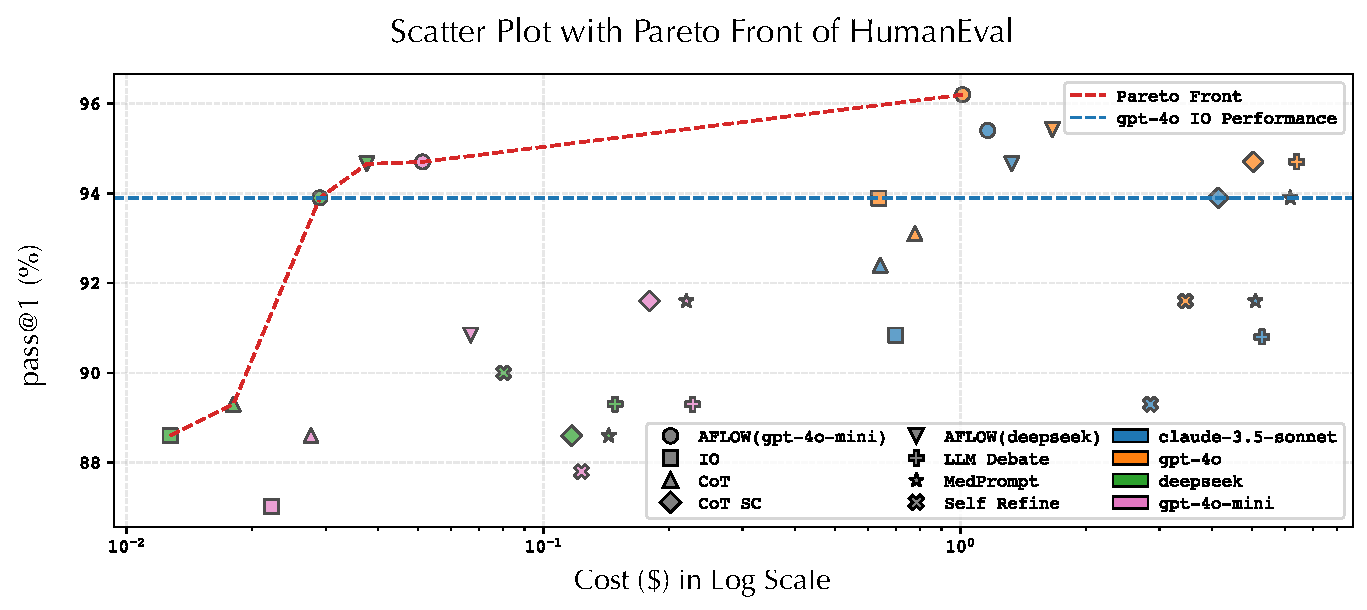
\includegraphics[width=\linewidth]{images/pareto_front.pdf}
  \label{fig:pareto}
  \vspace{-7mm}
  \caption{The cost refers to the total expense of executing the divided HumanEval test set. \model (execution model) refers to workflows found by \model using the execution model to obtain feedback. The colors in the legend represent the LLM used to execute each workflow in test dataset. The specific numerical values for this Figure can be found in Appendix \ref{appendix:cost}.}
  \vspace{-3mm}
\end{figure}

\noindent\textbf{Cost Analysis}  We demonstrate the comparison of performance and cost between the baselines and the top three workflows found by \model using GPT-4o-mini and DeepSeek-V2.5 as execution LLMs. The comparison is made across four models with different capabilities and price points. Results demonstrate that \model can identify workflows that allow weaker models to outperform stronger models on the pareto front of cost-effectiveness. This breakthrough effectively removes barriers to the widespread application of agentic workflows across various domains. By automating the design of effective agentic workflows, \model eliminates the human labor costs previously required. Moreover, the ability to achieve superior performance at lower costs compared to stronger models opens up further possibilities for widespread adoption.



\begin{figure}[h]
  \centering
  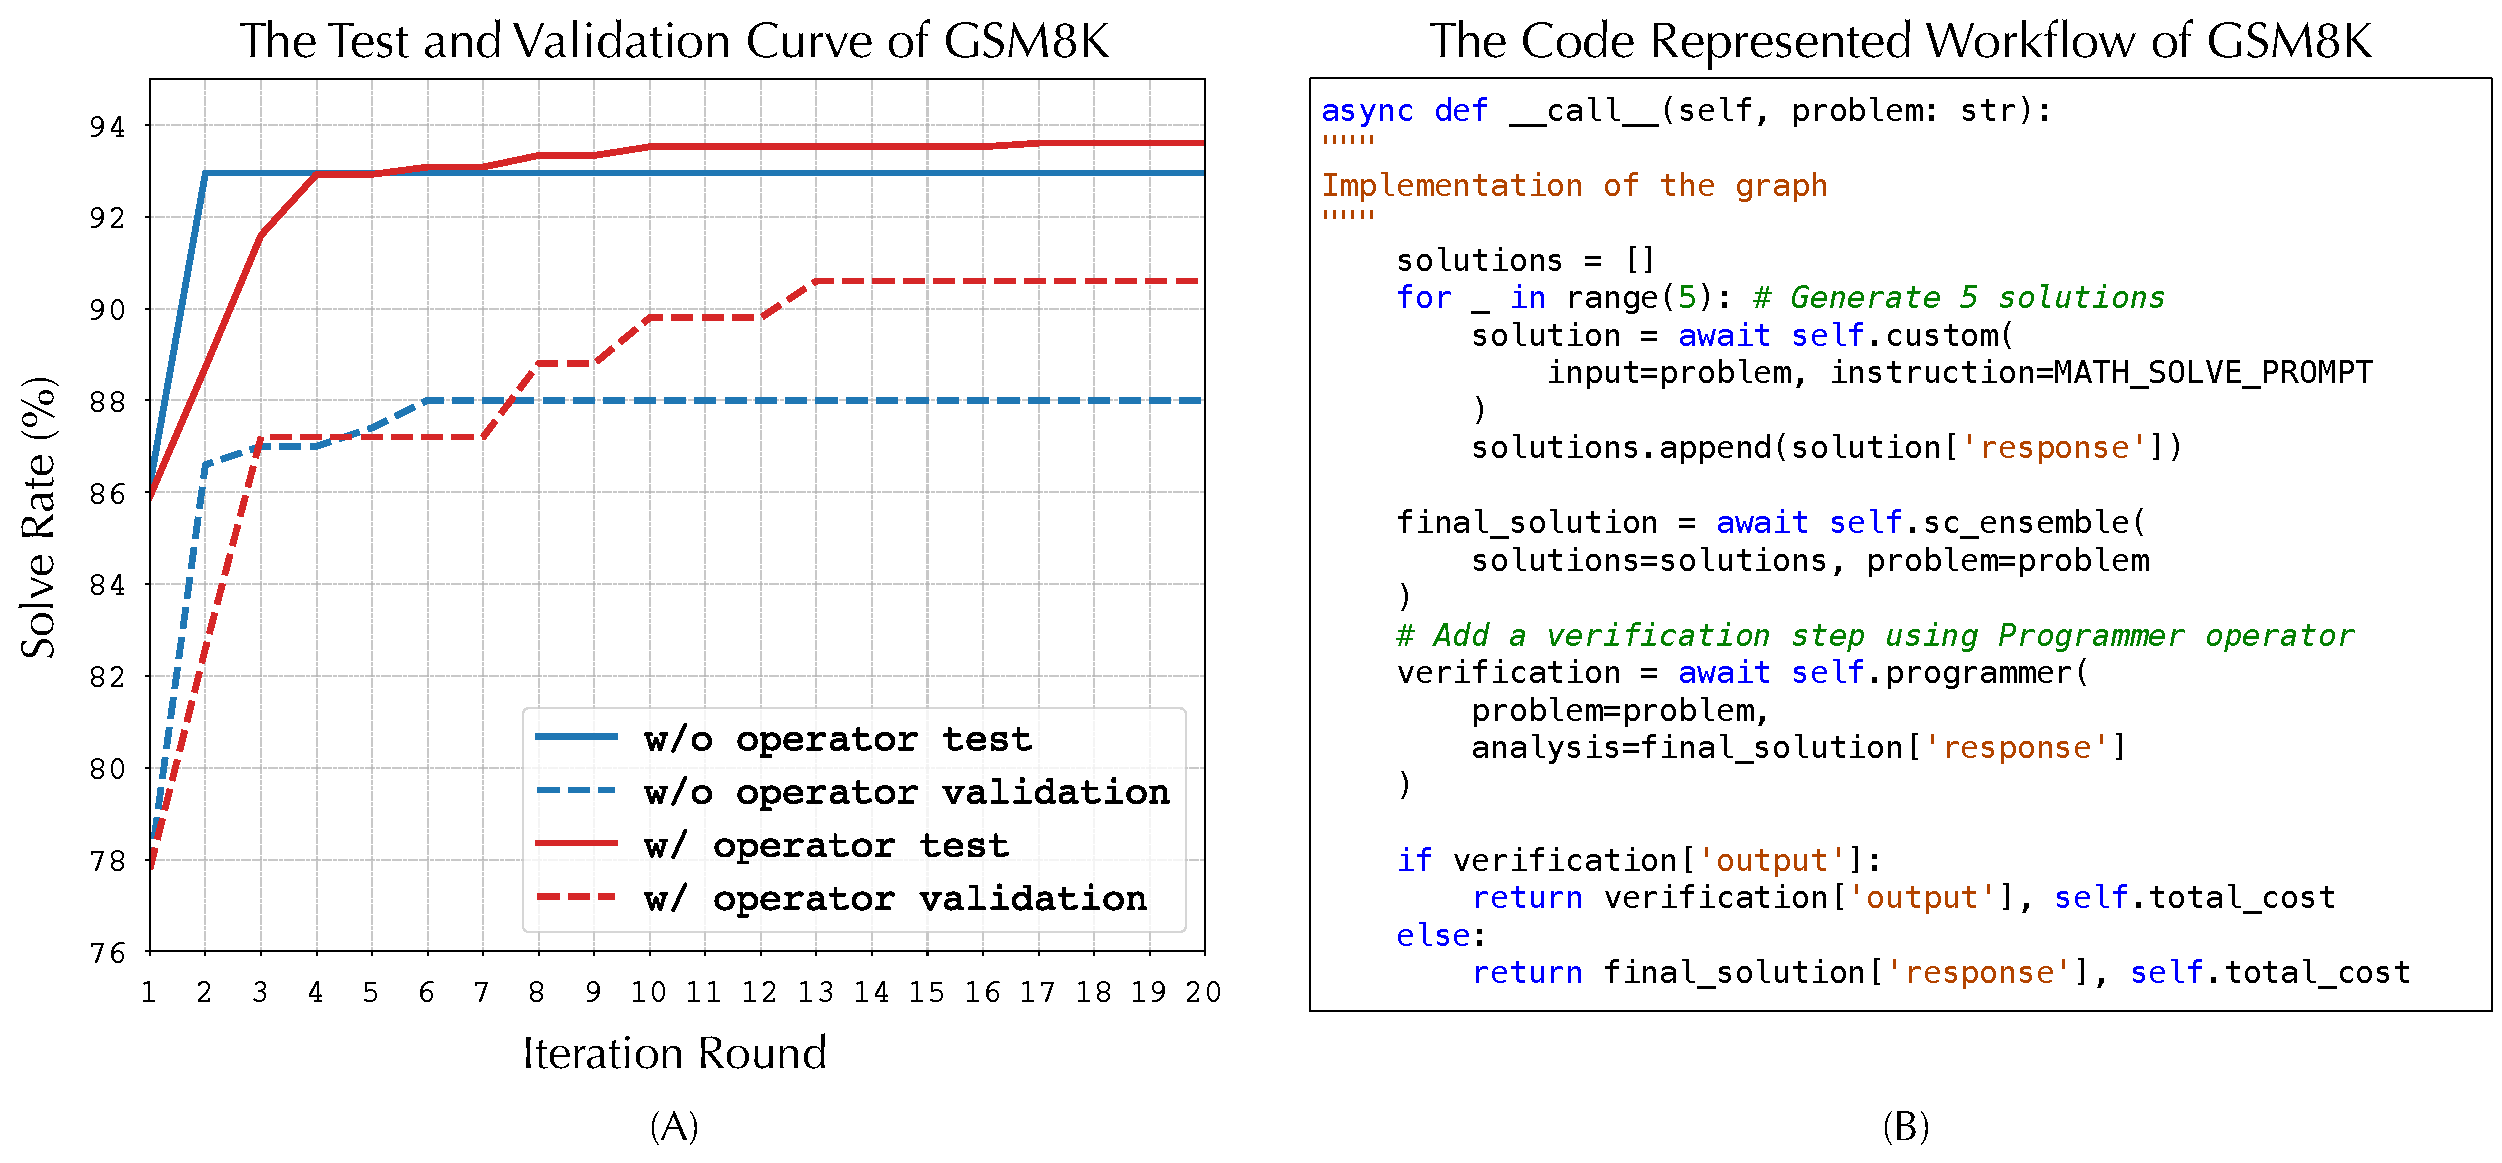
\includegraphics[width=\linewidth]{images/ablation_study.pdf}
  \vspace{-7mm}
  \caption{(A) Comparison of highest performance curves on GSM8K for both validation and test sets generated by \model with and without operators. Compared to other datasets, GSM8K has a larger data volume, meaning that the same percentage improvement represents a greater increase in correctly solved samples, avoiding fluctuations in improvement due to small data size that could affect comparisons; (B): The code for the best-performing workflow discovered by \model on the GSM8K dataset.}
  \label{fig:ablation}
  \vspace{-2mm}
\end{figure}

\noindent\textbf{Ablation Study}
\label{sec:ablation}
% To enhance search efficiency, we introduce operators into the search space, which can be viewed as a form of human design. To explore \model's performance with zero human intervention, we conducted an ablation study on the GSM8K dataset. Results shown in Figure~\ref{fig:ablation} demonstrate that \model with operators discover better-performing workflows within the same number of iterations, exhibiting a trend of multiple small improvements. This indicates that operators effectively boost search efficiency by introducing a constrained search space. Even without operators, \model still achieves 93.1\% performance, surpassing other manually designed methods.
We introduce operators as human-designed effort to enhance search efficiency. An ablation study on GSM8K (Figure~\ref{fig:ablation}) shows that operators help \model discover better workflows more efficiently, achieving incremental improvements. Notably, even without operators, \model maintains strong performance (93.1\%), surpassing manual designs. Notably, \model autonomously develops ensemble-like structures without operators, demonstrating its capability for independent workflow design and marking a significant step towards full automation. Details is shown in Appendix \ref{appendix:case_study}.

% As introduced in Section \ref{sub:design}, we incorporate operators into the search space to increase its search efficiency. When transferring to other tasks, the creation of operators can be seen as a human effort. To explore the performance of \model with zero human effort, we conduct an ablation experiment on the GSM8K dataset. As shown in Section~\ref{fig:ablation}, 

% % 带有Operator的曲线相比于不带Operator在相同的迭代轮次内搜索出了表现更好的workflow，并且整体曲线展示出幅度小但多次的上升。这说明了Operator的作用：Operator能够有效的提升搜索效率，因为这一结构将\model引入了有限制搜索空间，which means因为使用Opeartor能够带来效果提升，所以\model的树状搜索会更多围绕带有Operator有效的路径进行，相当于锁定了路径，所以提升了搜索效率。而在without operators, \model still demonstrates good optimization performance, pushing the performance to 93.1\%, surpassing the compared mannually designed methods.

% The second observation is that despite having no pre-prompts, the experiment without operators developed interfaces similar to ensemble and formatting during the iteration process. This proves the advantages of using LLM as an optimizer to search code-represented edges, enabling it to independently design efficient structures for problems. Some workflows that appeared in the ablation experiments are shown in \ref{}.



\begin{figure}[htbp]
  \centering
  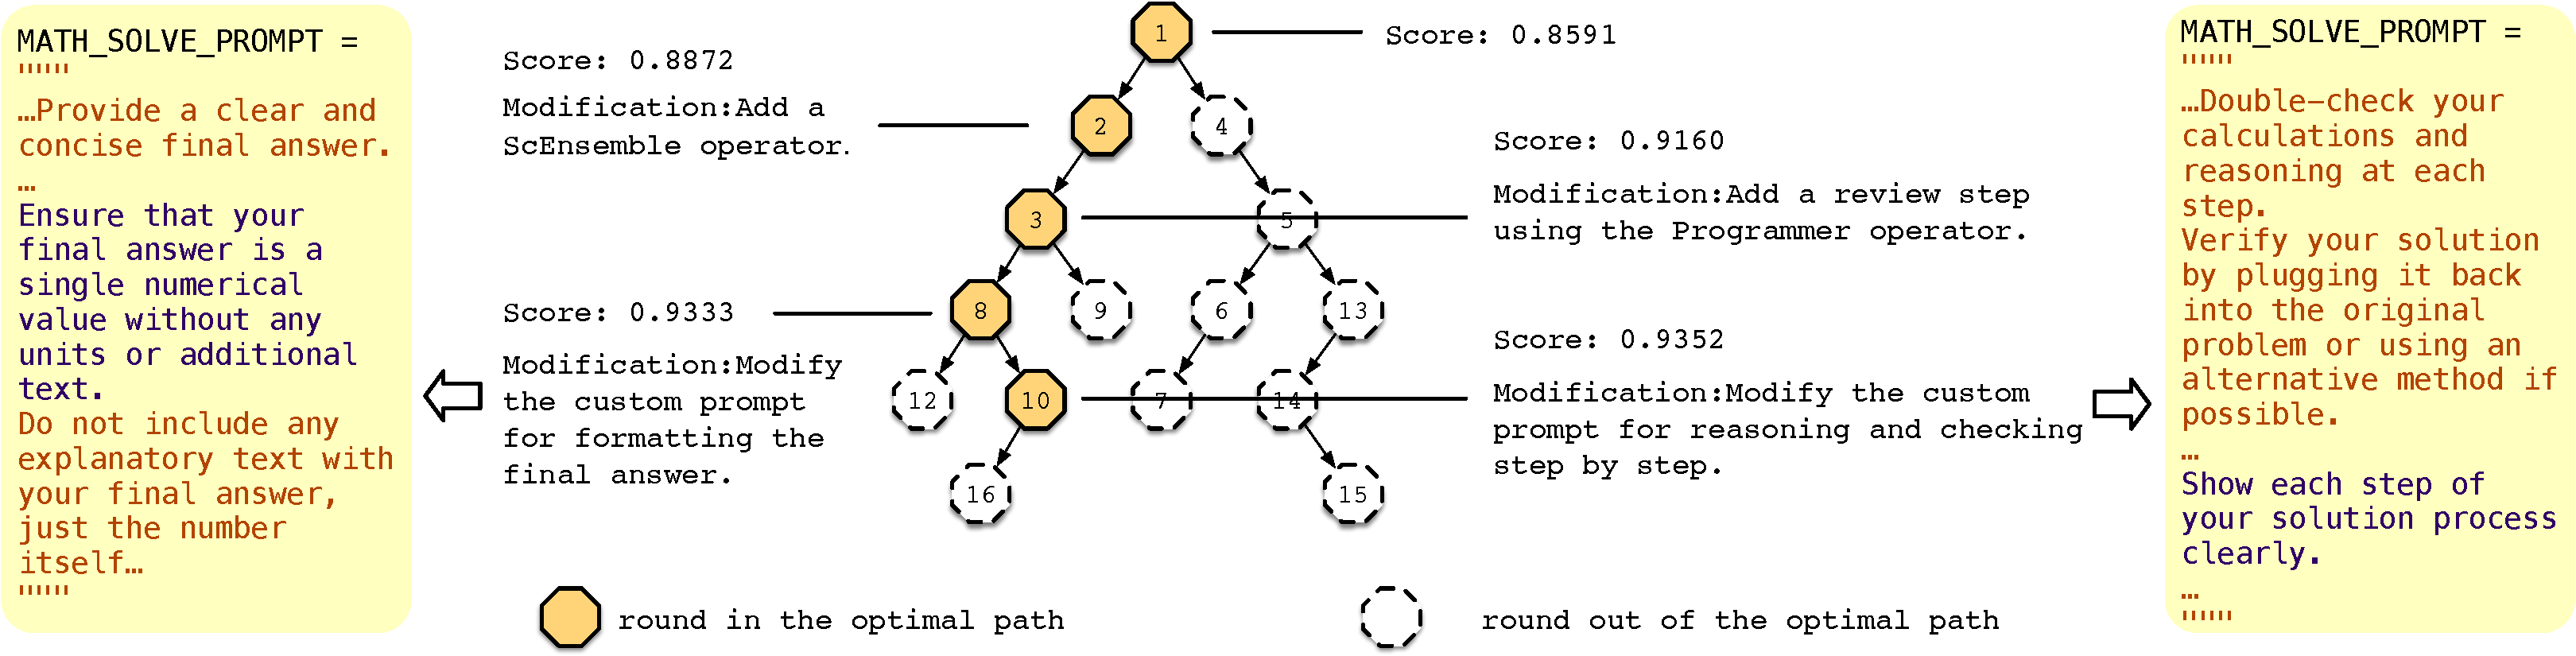
\includegraphics[width=\linewidth]{images/case_study.pdf}
  \vspace{-7mm}
  \caption{Tree-structured iteration process of \model on GSM8K: We highlight the path from the initial round (round 1) to the best-performing workflow, reporting the score for each node and its modification from the previous node. The purple sections in the prompts on both sides represent the main prompt modifications in this iteration.}
  \vspace{-3mm}
  \label{fig:casestudy}
\end{figure}

\noindent\textbf{Case Study}
\model demonstrates a clear iteration process, as shown in Figure \ref{fig:casestudy}, illustrating how it evolves from a blank template (containing only a single Node without prompts) to the structure presented in Figure \ref{fig:ablation}(B). In each iteration, \model employs a single-step modification, meaning it either adds one operator (rounds 2, 3) or makes a targeted modification to a prompt (rounds 8, 10). Among the unsuccessful exploration rounds, \model introduced a custom review node that directly modified answers generated through complex processes without additional reasoning (round 5), which decreased accuracy. In round 14, \model attempted to rephrase the problem but overly focused on ``discount'' information, leading to a decrease in accuracy. This iteration process showcases how tree-based search allows \model to further optimize known paths while retaining the ability to explore new ones. On the MBPP dataset, \model discovered structures similar to current manually designed workflows, such as test generation and execution by LLMs as seen in \citet{Tal2024Alpha}. The workflow and more discovered results are presented in Appendix \ref{appendix:case_study} and a complete optimization process is presented in Appendix \ref{sec:trajectory}.